\documentclass[../Main.tex]{subfiles}
\begin{document}

Lưu ý: \textbf{Trước khi viết ĐATN, sinh viên cần đọc kỹ hướng dẫn và quy định chi tiết} về cách viết ĐATN trong Phụ lục A.
Sinh viên tuân theo mẫu tài liệu này để viết báo cáo đồ án tốt nghiệp, vì tài liệu này đã được căn chỉnh, chỉnh sửa theo đúng chuẩn báo cáo kỹ thuật đồ án tốt nghiệp (ISO 7144:1986).
Sinh viên viết trực tiếp vào file này, chỉ chỉnh sửa nội dung, và không viết trên file mới.

\textbf{Khi đóng quyển ĐATN}, sinh viên cần lưu ý tuân thủ hướng dẫn ở phụ lục A.9

\textbf{SV cần đặc biệt lưu ý cách hành văn}.
Mỗi đoạn văn không được quá dài và cần có ý tứ rõ ràng, bao gồm duy nhất một ý chính và các ý phân tích bổ trợ để làm rõ hơn ý chính.
Các câu văn trong đoạn phải đầy đủ chủ ngữ vị ngữ, cùng hướng đến chủ đề chung.
Câu sau phải liên kết với câu trước, đoạn sau liên kết với đoạn trước.
Trong văn phong khoa học, sinh viên không được dùng từ trong văn nói, không dùng các từ phóng đại, thái quá, các từ thiếu khách quan, thiên về cảm xúc, về quan điểm cá nhân như “tuyệt vời”, “cực hay”, “cực kỳ hữu ích”, v.v.
Các câu văn cần được tối ưu hóa, đảm bảo rất khó để thể thêm hoặc bớt đi được dù chỉ một từ.
Cách diễn đạt cần ngắn gọn, súc tích, không dài dòng.

Mẫu ĐATN này được thiết kế phù hợp nhất với đa số các đề tài xây dựng phần mềm ứng dụng.
Với các dạng đề tài khác (giải pháp, nghiên cứu, phần mềm đặc thù, v.v.)
, sinh viên dựa trên cấu trúc và hướng dẫn của báo cáo này để đề xuất và trao đổi với giáo viên hướng dẫn để thiết kế khung báo cáo đồ án cho phù hợp.
Sinh viên lưu ý \textbf{trong mọi trường hợp, SV luôn phải sử dụng định dạng báo cáo này, và phải đọc kỹ toàn bộ các hướng dẫn từ đầu tới cuối.
}
Các hướng dẫn không chỉ áp dụng riêng cho đề tài ứng dụng, mà còn phù hợp với các dạng đề tài khác.
Ngoài ra, trong mẫu ĐATN này đã được tích hợp một số hướng dẫn dành riêng cho đề tài nghiên cứu.

Chương 1 có độ dài từ 3 đến 6 trang với các nội dung sau đây

\section{Problem}
\label{sec:problem}

Today, as society continues to develop, many workers and students are moving away from home to work or study, making it crucial to find accommodation near their workplace or school.
Not every work area or school has enough dormitories for workers or students, especially during hot, rainy, or cold days, which causes inconvenience and difficulty in finding rental rooms, particularly for students and even for working individuals.

Information technology, and especially the Internet, has transformed the way people live, communicate, work, and access diverse and fast information sources.
The advent of the Internet has become a powerful tool for those looking for resources in general or searching for rental rooms in particular, making it easier than ever.
For those in need of renting accommodation, traditional search methods can be challenging, time-consuming, and labor-intensive to find rooms that meet their criteria.
For landlords, reaching potential tenants is quite challenging due to location and limited communication methods.
Now, with the advent of network systems, just a computer connected to the internet allows us to post and search for rental rooms anywhere, with prices suitable to our needs easily.

From these reasons, I decided to choose the topic ``Building a website to Finding Rental Rooms''.
With the desire to create a website that supports users in posting and searching for rental rooms that match their needs.

\section{Purpose and requirements}
\label{sec:purpose}

\subsection{Purpose}

Currently, there are many websites and applications on the internet that help users search for and post rental listings, such as phongtro123.com, nhatot.com, and ohanaliving.vn.
While these websites generally meet the functional requirements of a rental search platform, they share a common issue: the cost of posting listings is too high.
Landlords have to pay a significant fee to list their rentals on these websites.

Based on the user need for posting and searching for rental information, I propose a solution: building a website to support rental searches.
This website will enable landlords to post their rental listings at a very low cost and allow those seeking rentals to search for rooms for free.
The website will cater to the majority of users looking for rental accommodations today.
Additionally, the website will provide functionalities for administrators to manage all system information, such as user accounts, rental listings, and revenue.
It will also offer landlords features such as posting listings, managing rooms, and managing posts.

The rental search website will provide a large amount of information about houses and rooms available for rent.
Visitors to the site can use search functions to find rentals by area, such as city or district, by specific address, by rental price, and by amenities offered.

Furthermore, the website will provide detailed information about the available rentals, including addresses, email contacts, and phone numbers, allowing users to contact landlords directly.

\subsection{Requirements}

\begin{itemize}
    \item Develop a simple, user-friendly interface that is easy to use.
    \item Research and understand the essential information needed for a rental listing.
    \item Gather requirements from real users to determine what information they need about a rental room.
    \item Clearly specify requirements.
    \item Design the system specification using an object-oriented approach for easy development.
    \item Implement the system using a RESTful API approach to facilitate easy upgrades and maintenance when issues arise.
    \item Build a complete website with all necessary features.
\end{itemize}

\section{Research situations}
\label{section:research}

Renting accommodation has always been a perennial issue.
Every year, hundreds of thousands of students from various provinces across the country come to study at universities, colleges, and vocational schools.
Additionally, many employees working far from home also need to rent houses or rooms.
However, the dormitory facilities at schools or companies can only meet the needs of less than 10\% of the students and employees.
The remaining students and employees have to face the challenge of finding rental accommodation near their study or work areas, which are often very expensive and do not meet the required quantity or quality of living conditions.

Hanoi is one of the cities with the highest density of universities in the country, attracting tens of thousands of students from all over to study.
Although many universities have their own dormitories and the city has student housing, not all students qualify to live there.
Additionally, some students, either because they have the financial means or because they want to live more comfortably and not be constrained by dormitory regulations, choose to seek off-campus housing.

With the significant increase in the number of students, the demand for rental accommodation in Hanoi is rising, making the student rental market extremely dynamic and competitive.
This has led to a shortage of available rentals and fierce price competition among landlords.
As a new academic year approaches, rental prices in areas near top universities are significantly higher compared to other areas.
One of the main challenges for students in finding rental accommodation is the quality and amenities of the rooms.
Due to high demand, many rental properties fail to meet the standards for security, hygiene, fire safety, and basic amenities.
Students often have to compromise between affordable rent and quality of living conditions.

In January 2024, Vietnam had a total of 78.44 million Internet users, with an Internet penetration rate of 79.1\% of the total population.
Analysis by Kepios indicates that the number of Internet users in Vietnam increased by an additional 502 thousand (+0.6\%) from January 2023 to January 2024.
This growth underscores the increasing number of Internet users, leading to a higher demand for accessing rental accommodation information.
Therefore, using websites to search for rental accommodations has completely replaced traditional methods, which is entirely reasonable and aligned with current trends.

Some websites support finding accommodations in Vietnam:

\begin{itemize}
    \item Website phongtro123.com
          \begin{figure}[H]
              \centering
              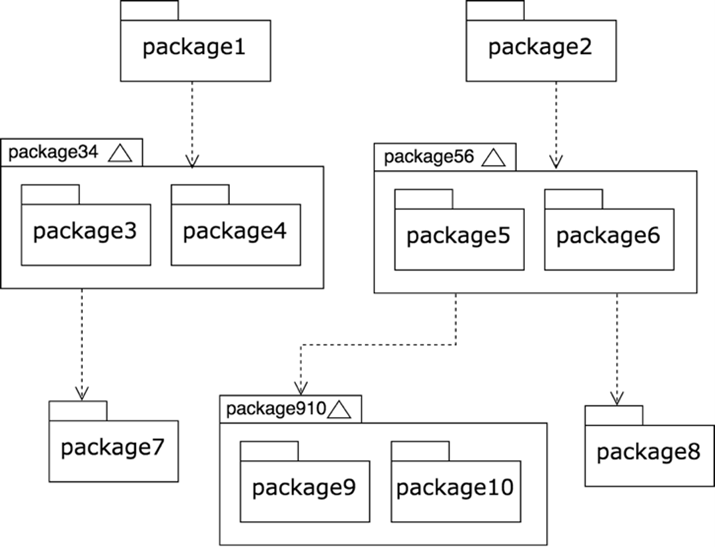
\includegraphics[width=\textwidth]{Figure/Picture1.png}
              \caption{Website phongtro123.com}
              \label{fig:phongtro123}
          \end{figure}
    \item Website nhatot.com
          \begin{figure}[H]
              \centering
              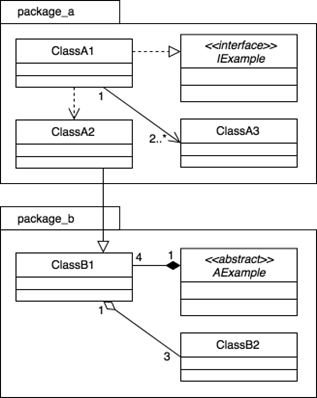
\includegraphics[width=\textwidth]{Figure/Picture2.png}
              \caption{Website nhatot.com}
              \label{fig:nhatot}
          \end{figure}
    \item Website ohanaliving.vn
          \begin{figure}[H]
              \centering
              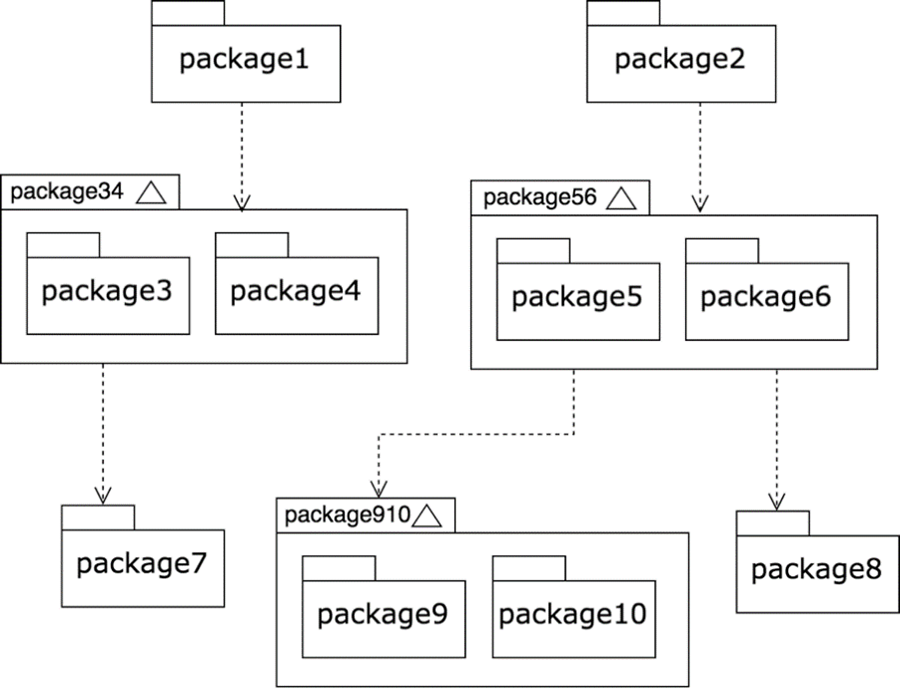
\includegraphics[width=\textwidth]{Figure/Picture3.png}
              \caption{Website ohanaliving.vn}
              \label{fig:ohanaliving}
          \end{figure}
\end{itemize}

\subsection{The importance of this topic}

The demand for accommodation for students and workers has been a persistent and challenging issue for many years, especially with the increasing number of students and workers studying or working far from home nowadays.
Finding satisfactory rental accommodations is difficult due to the rise of fraudulent listings.
Scammers take advantage of renters' vulnerabilities to deceive them into paying deposits or inflate rental prices through intermediaries who sublet at exorbitant rates, making it financially burdensome for many to secure housing.

Providing solutions to the housing issue for workers and students not only improves quality of life but also contributes to the overall socio-economic development of the country.

The ``Accommodation Search Support'' website is created to directly connect renters and landlords without intermediaries, offering affordable fees for listings.
It provides accurate and quick information for renters to find accommodation within desired price ranges and locations.
This platform helps renters find housing without the need for extensive travel to search for rental properties.

Therefore, this topic is not only highly relevant but also holds significant importance for the community, contributing to improving living conditions and reducing difficulties in finding accommodations for students and workers in Vietnam.

\section{Motivation}
\label{section:1.1}
Khi đặt vấn đề, sinh viên cần làm nổi bật mức độ cấp thiết, tầm quan trọng và/hoặc quy mô của bài toán của mình.

Gợi ý cách trình bày cho sinh viên: Xuất phát từ tình hình thực tế gì, dẫn đến vấn đề hoặc bài toán gì.
Vấn đề hoặc bài toán đó, nếu được giải quyết, đem lại lợi ích gì, cho những ai, còn có thể được áp dụng vào các lĩnh vực khác nữa không.
Sinh viên cần lưu ý phần này chỉ trình bày vấn đề, tuyệt đối không trình bày giải pháp.

\section{Objectives and scope of the graduation thesis}
\label{section:1.2}
Sinh viên trước tiên cần trình bày tổng quan các kết quả của các nghiên cứu hiện nay cho bài toán giới thiệu ở phần \ref{section:1.1} (đối với đề tài nghiên cứu), hoặc về các sản phẩm hiện tại/về nhu cầu của người dùng (đối với đề tài ứng dụng).
Tiếp đến, sinh viên tiến hành so sánh và đánh giá tổng quan các sản phẩm/nghiên cứu này.

Dựa trên các phân tích và đánh giá ở trên, sinh viên khái quát lại các hạn chế hiện tại đang gặp phải.
Trên cơ sở đó, sinh viên sẽ hướng tới giải quyết vấn đề cụ thể gì, khắc phục hạn chế gì, phát triển phần mềm \textbf{có các chức năng chính gì}, tạo nên đột phá gì, v.v.

Trong phần này, sinh viên lưu ý chỉ trình bày tổng quan, không đi vào chi tiết của vấn đề hoặc giải pháp.
Nội dung chi tiết sẽ được trình bày trong các chương tiếp theo, đặc biệt là trong Chương 5.

\section{Tentative solution}
\label{section:1.3}
Từ việc xác định rõ nhiệm vụ cần giải quyết ở phần \ref{section:1.2}, sinh viên đề xuất định hướng giải pháp của mình theo trình tự sau: (i) Sinh viên trước tiên trình bày sẽ giải quyết vấn đề theo định hướng, phương pháp, thuật toán, kỹ thuật, hay công nghệ nào; Tiếp theo, (ii) sinh viên mô tả ngắn gọn giải pháp của mình là gì (khi đi theo định hướng/phương pháp nêu trên); và sau cùng, (iii) sinh viên trình bày đóng góp chính của đồ án là gì, kết quả đạt được là gì.

Sinh viên lưu ý không giải thích hoặc phân tích chi tiết công nghệ/thuật toán trong phần này.
Sinh viên chỉ cần nêu tên định hướng công nghệ/thuật toán, mô tả ngắn gọn trong một đến hai câu và giải thích nhanh lý do lựa chọn.

\section{Thesis organization}
\label{section:1.4}
Phần còn lại của báo cáo đồ án tốt nghiệp này được tổ chức như sau.

Chương 2 trình bày về v.v.

Trong Chương 3, em/tôi giới thiệu về v.v.

\textbf{Chú ý:}
Sinh viên cần viết mô tả thành đoạn văn đầy đủ về nội dung chương.
Tuyệt đối không viết ý hay gạch đầu dòng.
Chương 1 không cần mô tả trong phần này.

Ví dụ tham khảo mô tả chương trong phần bố cục đồ án tốt nghiệp: Chương *** trình bày đóng góp chính của đồ án, đó là một nền tảng ABC cho phép khai phá và tích hợp nhiều nguồn dữ liệu, trong đó mỗi nguồn dữ liệu lại có định dạng đặc thù riêng.
Nền tảng ABC được phát triển dựa trên khái niệm DEF, là các module ngữ nghĩa trợ giúp người dùng tìm kiếm, tích hợp và hiển thị trực quan dữ liệu theo mô hình cộng tác và mô hình phân tán.

\textbf{Chú ý:}
Trong phần nội dung chính, mỗi chương của đồ án nên có phần Tổng quan và Kết chương.
Hai phần này đều có định dạng văn bản “Normal”, sinh viên không cần tạo định dạng riêng, ví dụ như không in đậm/in nghiêng, không đóng khung, v.v.

Trong phần Tổng quan của chương N, sinh viên nên có sự liên kết với chương N-1 rồi trình bày sơ qua lý do có mặt của chương N và sự cần thiết của chương này trong đồ án.
Sau đó giới thiệu những vấn đề sẽ trình bày trong chương này là gì, trong các đề mục lớn nào.

Ví dụ về phần Tổng quan: Chương 3 đã thảo luận về nguồn gốc ra đời, cơ sở lý thuyết và các nhiệm vụ chính của bài toán tích hợp dữ liệu.
Chương 4 này sẽ trình bày chi tiết các công cụ tích hợp dữ liệu theo hướng tiếp cận “mashup”.
Với mục đích và phạm vi của đề tài, sáu nhóm công cụ tích hợp dữ liệu chính được trình bày bao gồm: (i) nhóm công cụ ABC trong phần 4.1, (ii) nhóm công cụ DEF trong phần 4.2, nhóm công cụ GHK trong phần 4.3, v.v.

Trong phần Kết chương, sinh viên đưa ra một số kết luận quan trọng của chương.
Những vấn đề mở ra trong Tổng quan cần được tóm tắt lại nội dung và cách giải quyết/thực hiện như thế nào.
Sinh viên lưu ý không viết Kết chương giống hệt Tổng quan.
Sau khi đọc phần Kết chương, người đọc sẽ nắm được sơ bộ nội dung và giải pháp cho các vấn đề đã trình bày trong chương.
Trong Kết chương, Sinh viên nên có thêm câu liên kết tới chương tiếp theo.

Ví dụ về phần Kết chương: Chương này đã phân tích chi tiết sáu nhóm công cụ tích hợp dữ liệu.
Nhóm công cụ ABC và DEF thích hợp với những bài toán tích hợp dữ liệu phạm vi nhỏ.
Trong khi đó, nhóm công cụ GHK lại chứng tỏ thế mạnh của mình với những bài toán cần độ chính xác cao, v.v.
Từ kết quả nghiên cứu và phân tích về sáu nhóm công cụ tích hợp dữ liệu này, tôi đã thực hiện phát triển phần mềm tự động bóc tách và tích hợp dữ liệu sử dụng nhóm công cụ GHK.
Phần này được trình bày trong chương tiếp theo – Chương 5.

\end{document}
